\section{System's Perspective}

\subsection{Design and Architecture}
Figure \ref{fig:systemoverview} provides an overview of our system infrastructure:
\begin{figure}[H]
    \centering
    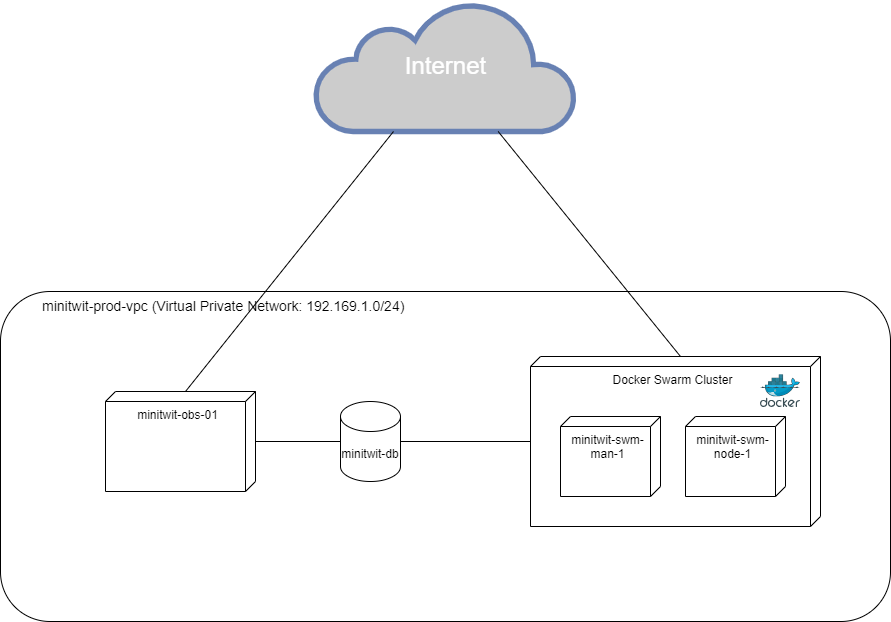
\includegraphics[width=0.7\linewidth]{images/system-overview.png}
    \caption{Overview of the system}
    \label{fig:systemoverview}
\end{figure}
The system includes a single Virtual Private Network with an IP 192.168.1.0/24. Within this network, we operate a database cluster consisting of a single node. This node is connected to the Docker Swarm cluster, featuring both a manager and a worker node.

Both our monitoring and cluster servers are visibly exposed to the internet. Additionally, the database server is accessible from the internet but has constraints to only talk to our servers and therefore not accept requests from any other host.

\subsection{Interactions of Subsystems}
Our system consists of three subsystems, namely SimulatorAPI, Minitwit, and Minitwit.Infrastructure. The SimulatorAPI and Minitwit subsystems, as can be seen in figure \ref{fig:subsystem-interaction}, are similar in structure, but differ since SimulatorAPI is a REST service and Minitwit is a website. Both controllers use the package in the subsystem Minitwit.Infrastructure to query for data using the Repository pattern.
%cite

\begin{figure}[H]
    \begin{center}
        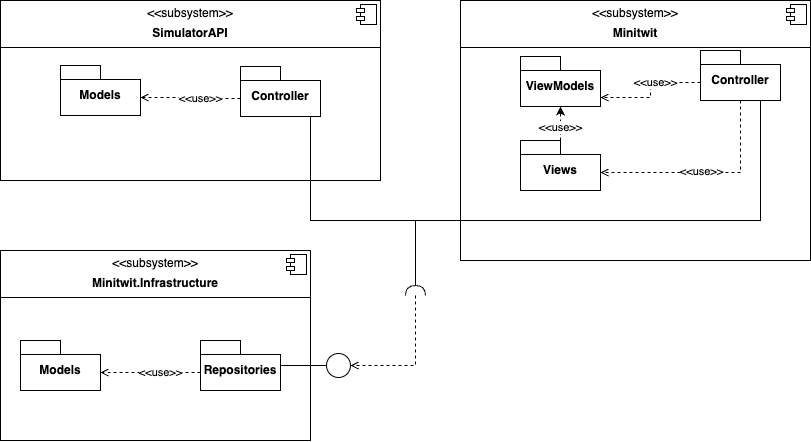
\includegraphics[width=1\textwidth]{Subsystem-Interaction.png}
    \end{center}
    \caption{An overview of the subsystems and how they interact}
    \label{fig:subsystem-interaction}
\end{figure}

As can be seen in figure \ref{fig:frontend-interaction} the controller for Minitwit handles a lot of logic in order to present the correct information to the user. However for SimulatorAPI, in figure \ref{fig:backend-interaction} there is little to non logic, and it only calls the repository to fetch the user messages.
\begin{figure}[H]
    \begin{center}
        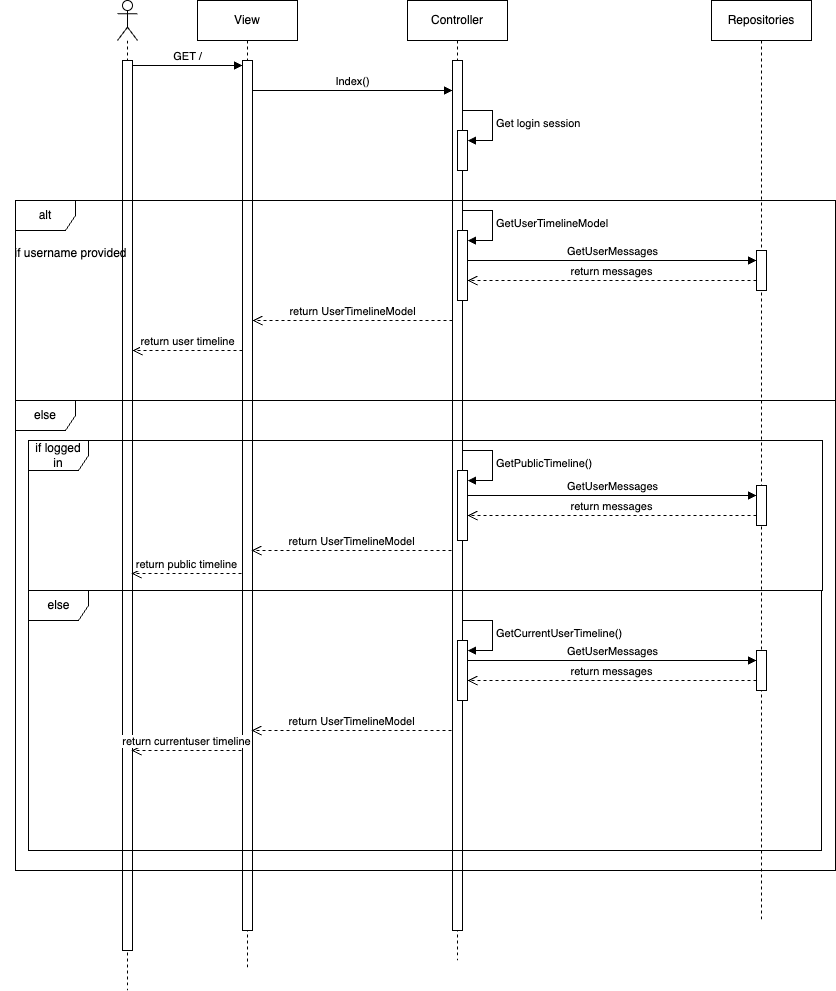
\includegraphics[width=1\textwidth]{Fronted-Sequence-Diagram.png}
    \end{center}
    \caption{Minitwit: Sequence diagram of a user call to the index page}
    \label{fig:frontend-interaction}
\end{figure}
\begin{figure}[H]
    \begin{center}
        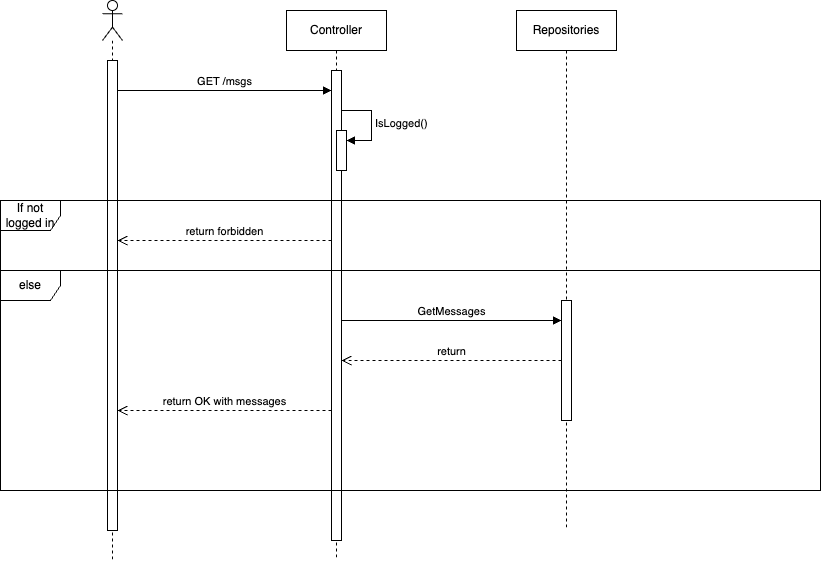
\includegraphics[width=1\textwidth]{Backend-Sequence-Diagram.png}
    \end{center}
    \caption{SimulatorAPI: Sequence diagram of a user call to get messages}
    \label{fig:backend-interaction}
\end{figure}
\subsubsection{Minitwit.Infrastructure}
In the previous section we saw that the controller logic is very different but needs to call the same queries.
Minitwit.Infrastructure is implemented to share duplicate code between the SimulatorAPI and Minitwit. This can be seen with the interaction of the package Repositories which leverages the Repository Pattern to abstract the logic of handling database queries and make it testable.


\subsection{Current state}
Table \ref{current-table} describes the status of the system after the simulator has been shut down.
\begin{table}[H]
    \begin{center}
        \begin{tabular}{ |c|c| }
            \hline
            Total requests & 34233 \\
            \hline
            Requests secured & 34233 \\
            \hline
            Total unhandled exceptions & 18 \\
            \hline
            P99 min response time & 94.2 ms \\
            \hline
            P99 max response time & 716 ms \\
            \hline
            Number of users &  116995\\
            \hline
            Avg followers per user &  28.5\\
            \hline
        \end{tabular}
    \end{center}
    \caption{System metrics}
    \label{current-table}
\end{table}
Furthermore, the static analysis tool Sonarcloud assesses that the quality of the overall code is good (see appendix \ref{appendix:sonarcloud}).
